% Chapter 4

\chapter{Análisis} % Main chapter title


\label{Chapter4} % Change X to a consecutive number; for referencing this chapter elsewhere, use \ref{ChapterX}

En este capítulo se realiza el análisis de las diversas aplicaciones de dispositivos IoT y su implementación en redes de comunicaciones móviles 5G. Se comienza con una breve descripción de estas tecnologías, y después se profundiza en el caso de uso mMTC donde se mencionan los escenarios más comunes de implementación, su clasificación y sus características, además se revisa el estándar actual (NB-IoT\footnote{ Muchos\ de\ los\ modelos\ aqu\textrm{í}\ propuestos\ est\textrm{á}n\ basados\ en\ trabajos\ de\ la\ 3GPP,\ como\ se\ revis\textrm{ó}\ en\ el Capítulo \ref{Chapter2},\ la\ 3GPP,\ es\ una\ organizaci\textrm{ó}n\ que\ est\textrm{á}\ respaldada\ por\ organismos\ alrededor\ de\ todo\ el\ mundo,\ adem\textrm{á}s\ de\ que\ se\ trata\ del\ grupo\ que\ estandariza\ tecnolog\textrm{í}as\ como\ LTE-M\ y\ NB-IoT,\ de\ manera\ que\ es\ una\ indudable\ referencia\ en\ su\ ahora\ inmersi\textrm{ó}n\ en\ la\ estandarizaci\textrm{ó}n\ de\ 5G.}) que cumple con los requisitos para la implementación de mMTC. Finalmente también se revisan los KPIs propuestos para este tipo de escenarios.\newline

Por último, se detallan cuáles son los modelos y técnicas que se usan para caracterizar el modelo de despliegue, canal y de tráfico de dispositivos IoT en redes 5G y además se presenta la actual propuesta de técnica de acceso múltiple al medio no ortogonal (NOMA) y su enfoque hacia un entorno masivo de dispositivos (con el uso de \textit{clusterización}).

%----------------------------------------------------------------------------------------
%	SECTION 
%----------------------------------------------------------------------------------------

\section{REDES 5G/IoT}

Aunque gran parte de la comunicación IoT se ha implementado hasta el momento, no se ha considerado para una conectividad masiva y una mejor eficiencia energética. \newline

IoT en los sistemas 5G tendrán un importante papel en esta generación futura ya que abrirán una puerta para una nueva arquitectura inalámbrica y servicios inteligentes. La reciente red celular LTE (4G) no será lo suficientemente eficiente para satisfacer las demandas de conectividad de múltiples dispositivos y velocidad de datos, calidad de servicio (QoS) de baja latencia y baja interferencia. Para abordar estos desafíos, 5G es la tecnología más prometedora \parencite{Chetri2020}. \newline

Por lo tanto, la comunicación masiva de tipo máquina (mMTC), será uno de los principales habilitadores clave para el despliegue de redes 5G-IoT.

%----------------------------------------------------------------------------------------
%	SECTION 
%----------------------------------------------------------------------------------------

\section{CLASIFICACIÓN Y ANÁLISIS DE LOS ÁMBITOS DE IoT}

La contribución en cuanto a la categorización de las aplicaciones de IoT que ya existen y las que se comenzarán a ver en años próximos, es vasta y no siempre compatible dependiendo del grupo que se consulte, de manera que se tomó como referencia el trabajo realizado en \parencite{NetTrafficIoT} como guía para los servicios que se espera brinden los nodos IoT en distintos ámbitos.\newline

La mayor parte del artículo \parencite{NetTrafficIoT}, los autores se dedicaron a la caracterización de las aplicaciones de IoT y sus dominios, los cuales se pueden dividir en 8, específicamente: edificios inteligentes y vivienda (\textit{Smart buildings and living}), cuidado de la salud inteligente (\textit{Smart healthcare}), medio ambiente inteligente (\textit{Smart environment}), ciudades inteligentes (\textit{Smart city}), energía inteligente (\textit{Smart energy}), transporte y movilidad  inteligentes (\textit{Smart transport and mobility}), fabricación y venta inteligentes (\textit{Smart manufacturing and retail}), agricultura inteligente (\textit{Smart agriculture}). Para cada uno de los dominios se especifican aplicaciones típicas que se podrían encontrar, sus características de tráfico, las tecnologías de red más adecuadas para darles servicio entre otras cosas.\newline

La primera parte del análisis correspondió a la selección de los dominios que resultasen adecuados para el sistema que se diseña, es decir los dominios cuya red que les brindará servicio primordialmente será una red de área amplia de bajo consumo (LPWAN, \textit{Low Power Wide Area Network}). Esto se debe a que algunas de las aplicaciones en los dominios antes mencionados están pensadas para redes de distintas características en las que tecnologías como RFID, \textit{Bluetooth }o \textit{ZigBee }podrían ser una mejor solución. A continuación se presenta la caracterización de cada uno de los dominios que en \parencite{NetTrafficIoT} se consideran viables para redes LPWAN.\newline

\subsection{Ciudades inteligentes \textit{(Smart City)}:}

Con el rápido incremento de la población y su concentración en poblaciones urbanas, se ha convertido en una prioridad la reducción del uso de recursos públicos, así como la reducción de costos de operación del día a día de una ciudad, ambas de la manera más óptima posible. Las aplicaciones en este dominio tratan justamente de abordar estos problemas y los servicios que brindan son bastante variados, los ejemplos van desde el control de luminarias hasta el manejo de desechos, estos y otros  pueden encontrarse en la \textit{Tabla~\ref{tab:smartcity}}, acompañados de más información tal como la caracterización de su tráfico y su demanda de QoS.\newline

\begin{table}
\caption{Características de las aplicaciones de Ciudades Inteligentes}
\label{tab:smartcity}
\centering
\begin{tabular}{*{5}{m{3cm}}}\\
\textbf{\textit{Servicio}} & \textbf{\textit{Tamaño de red}} & \textbf{\textit{Tasa de tráfico}} & \textbf{\textit{Demanda de QoS}} & \textbf{\textit{Fuente de energía}} \\ \hline \hline
\textit{Monitoreo del consumo de agua y electricidad en la ciudad} & \footnotesize{Media a grande, cientos a miles de dispositivos} & \footnotesize{Periódico, 1 msj cada 10 min por dispositivo} & \footnotesize{Baja, tolerante al retardo 1 min} & \footnotesize{Alimentado por la red eléctrica/ autoalimentado} \\ \hline
\textit{Control de iluminación} & \footnotesize{Grande, miles de dispositivos} & \footnotesize{Aleatorio, poco frecuente} & \footnotesize{Media, tolerante al retardo 15 seg} & \footnotesize{Alimentado por la red eléctrica }\\ \hline
\textit{Vigilancia de estacionamientos} & \footnotesize{Grande, miles de dispositivos} & \footnotesize{Aleatorio, poco frecuente} & \footnotesize{Media, tolerante al retardo 10 seg} & \footnotesize{Alimentado por batería }\\ \hline
\textit{Control del tráfico} & \footnotesize{Grande, miles de dispositivos} & \footnotesize{Periódico, 1 msj cada 10 min por dispositivo, aleatorio para alarmas} & \footnotesize{Media, tolerante al retardo 15 seg, alta para alarmas} & \footnotesize{Alimentado por batería} \\ \hline
\textit{Mantenimiento de deshechos} & \footnotesize{Grande, miles de dispositivos} & \footnotesize{Aleatorio, poco frecuente} & \footnotesize{Media, tolerante al retardo 30 seg} & \footnotesize{Alimentado por batería }\\ \hline
\textit{Monitoreo de condiciones urbanas} & \footnotesize{Media a grande, cientos a miles de dispositivos} & \footnotesize{Periódico, 1 msj cada 15 min por dispositivo, aleatorio para alarmas} & \footnotesize{Media, tolerante al retardo 30 seg, alta para alarmas} & \footnotesize{Alimentado por batería }\\ \hline
\textit{Monitoreo de la salud estructural de edificios} & \footnotesize{Media a grande, cientos a miles de dispositivos} & \footnotesize{Periódico, 1 msj cada 15 min por dispositivo, aleatorio para alarmas} & \footnotesize{Media, tolerante al retardo 30 seg, alta para alarmas} & \footnotesize{Alimentado por batería} \\ 
\end{tabular}
\end{table}

\subsection{Ambiente inteligente \textit{(Smart Environment)}}

Este dominio comprende las aplicaciones que se encargan de monitorear el ambiente a nuestro alrededor y lo que ocurre en él, y aunque no se pueda controlar la fuerza de la naturaleza, con una correcta observación se pueden detectar distintos fenómenos naturales y reaccionar a tiempo ante ellos. En el caso especial de eventos que podrían ocasionar una catástrofe, es importante reaccionar lo más rápido posible por lo que el brindar el servicio a algunas de las aplicaciones de este dominio se volverá crítico. En la \textit{Tabla~\ref{tab:smartenv}} podemos encontrar la caracterización de las aplicaciones consideradas en \parencite{NetTrafficIoT} para \textit{Ambiente Inteligente.}\newline


\begin{table}
\caption{Características de las aplicaciones de Ambiente Inteligente}
\label{tab:smartenv}
\centering
\begin{tabular}{*{5}{m{3cm}}} \\ 
\textbf{\textit{Servicio}} & \textbf{Tamaño de red} & \textbf{Tasa de tráfico} & \textbf{Demanda de QoS} & \textbf{Fuente de energía} \\ \hline 
\textit{Detección de incendios forestales}  & \footnotesize{ Media a grande, cientos a miles de dispositivos } & \footnotesize{ Aleatorio, poco frecuente } & \footnotesize{ Media, tolerante al retardo 15 seg } & \footnotesize{ Alimentado por batería } \\ \hline 
\textit{Detección de terremotos}  & \footnotesize{ Media a grande, cientos a miles de dispositivos } & \footnotesize{ Aleatorio, poco frecuente } & \footnotesize{ Alta, tolerante al retardo 5 seg } & \footnotesize{ Alimentado por batería } \\ \hline 
\textit{Detección de Tsunamis}  & \footnotesize{ Media a grande, cientos a miles de dispositivos } & \footnotesize{ Aleatorio, poco frecuente } & \footnotesize{ Alta, tolerante al retardo 5 seg } & \footnotesize{ Alimentado por batería } \\ \hline 
\textit{Detección de derrumbes y avalanchas}  & \footnotesize{ Media a grande, cientos a miles de dispositivos } & \footnotesize{ Aleatorio, poco frecuente } & \footnotesize{ Alta, tolerante al retardo 5 seg } & \footnotesize{ Alimentado por batería } \\ \hline 
\textit{Monitoreo de actividad volcánica}  & \footnotesize{ Pequeña, 10s de dispositivos } & \footnotesize{ Aleatorio, poco frecuente } & \footnotesize{ Alta, tolerante al retardo 5 seg } & \footnotesize{ Alimentado por batería } \\ \hline 
\textit{Monitoreo de la contaminación del aire } & \footnotesize{ Media a grande, cientos a miles de dispositivos } & \footnotesize{ Periódico, 1 msj cada 15 min por dispositivo } & \footnotesize{ Media, tolerante al retardo 15 seg } & \footnotesize{ Alimentado por batería } \\ \hline 
\textit{Rastreo de vida salvaje.}  & \footnotesize{ Media, cientos de dispositivos } & \footnotesize{ Periódico, 1 msj cada 30 min por dispositivo } & \footnotesize{ Baja, tolerante a unas horas } & \footnotesize{ Alimentado por batería } \\ 
\end{tabular}
\end{table}

\subsection{Energía inteligente \textit{(Smart Energy)}:}

El dominio de Energía Inteligente\textit{Smart Energy }se refiere a las mejoras en la distribución y el consumo de fuentes de energía o recursos necesarios, tales como la electricidad, el gas y el agua. Aunque el foco de atención está en la electricidad ya que existe una tendencia más marcada hacia su ahorro y la utilización de fuentes renovables. \newline

Los nodos de IoT para aplicaciones de este dominio podrían monitorear las condiciones cambiantes de la red, para posteriormente generar una reconfiguración apropiada del servicio. En la \textit{Tabla~\ref{tab:smartenergy}} podemos encontrar la caracterización descrita en \parencite{NetTrafficIoT} para distintas aplicaciones de Energía Inteligente.\newline

\begin{table}
\caption{Características de las aplicaciones de Energía Inteligente}
\label{tab:smartenergy}
\centering


\begin{tabular}{*{5}{m{3cm}}}  \\  
\textbf{\textit{Servicio}} & \textbf{Tamaño de red} & \textbf{Tasa de tráfico} & \textbf{Demanda de QoS} & \textbf{Fuente de energía} \\ \hline
\textit{Medición inteligente}  & \footnotesize{ Media a grande, 1 dispositivo por hogar } & \footnotesize{ Periódico, 1 msj cada 15 min por dispositivo } & \footnotesize{ Media, tolerante al retardo 15 seg } & \footnotesize{ Alimentado por la red eléctrica/ Baterías } \\ \hline 
\textit{Gestión de activos}  & \footnotesize{ Media a grande, cientos a miles de dispositivos } & \footnotesize{ Periódico, 1 msj cada 15 min por dispositivo } & \footnotesize{ Media, tolerante al retardo 15 seg } & \footnotesize{ Alimentado por la red eléctrica/ Baterías } \\ \hline 
\textit{Detección de interrupciones en el servicio } & \footnotesize{ Media a grande, 1 dispositivo por hogar } & \footnotesize{ Aleatorio, poco frecuente } & \footnotesize{ Alta, tiempo real } & \footnotesize{ Alimentado por la red eléctrica/ Baterías } \\ 
\end{tabular}
\end{table}

\subsection{Transporte y movilidad inteligentes \textit{(Smart Transport and Mobility)}:}

Tanto el crecimiento urbano como el crecimiento de las fuentes de transporte de pasajeros y de mercancías, con más frecuentes congestiones viales y una mayor movilidad requerida, han creado una demanda de administrar el transporte y la movilidad de una manera más inteligente. \newline

El objetivo de aplicaciones IoT en el dominio de Transporte y movilidad inteligentes\textit{ (Smart Transport and Mobility)}es ayudar a resolver el problema de movilidad tanto de pasajeros como de mercancías, haciéndolo más rápido, más barato y más seguro. En la \textit{Tabla~\ref{tab:smartrans}} se encuentra la caracterización presentada en \parencite{NetTrafficIoT} para distintas aplicaciones de este dominio.\newline

\begin{table}
\caption{Características de las aplicaciones de Transporte y Movilidad inteligentes}
\label{tab:smartrans}
\centering
\begin{tabular}{*{5}{m{3cm}}}\\ 
\textit{Servicio} & Tamaño de red & Tasa de tráfico & Demanda de QoS & Fuente de energía \\ \hline
\textit{Automatización de vehículos}  & \footnotesize{ Grande, miles de dispositivos } & \footnotesize{ Periódico, 1 msj cada 24 hrs por vehículo. } & \footnotesize{ Baja, tolerante al retardo 1 min } & \footnotesize{ Alimentado por batería del vehículo } \\ \hline 
\textit{Localización y monitoreo de vehículos}  & \footnotesize{ Grande, miles de dispositivos } & \footnotesize{ Periódico, 1 msj cada 30 seg por vehículo } & \footnotesize{ Media, tolerante al retardo 10 seg } & \footnotesize{ Alimentado por batería del vehículo } \\ \hline 
\textit{Monitoreo de la calidad del embarque}  & \footnotesize{ Media, cientos de dispositivos } & \footnotesize{ Periódico, 1 msj cada 15 min por dispositivo } & \footnotesize{ Media, tolerante al retardo 15 seg } & \footnotesize{ Alimentado por batería } \\ \hline 
\textit{Control dinámico de semáforos}  & \footnotesize{ Grande, miles de dispositivos } & \footnotesize{ Periódico, 1 msj cada min por dispositivo } & \footnotesize{ Alta, tolerante al retardo 5 seg } & \footnotesize{ Alimentado por la red eléctrica } \\ \hline 
\textit{Monitoreo de las condiciones del camino} & \footnotesize{ Grande, miles de dispositivos } & \footnotesize{ Aleatorio, poco frecuente } & \footnotesize{ Media, tolerante al retardo 30 seg } & \footnotesize{ Alimentado por batería } \\
\end{tabular}
\end{table}

%----------------------------------------------------------------------------------------
%	SECTION 
%----------------------------------------------------------------------------------------

\section{CARACTERÍSTICAS DEL ESCENARIO A IMPLEMENTAR}

Las distintas aplicaciones presentadas en la sección anterior pertenecen a varios dominios y estas muy seguramente se verán desplegadas en un futuro próximo en ciudades alrededor de todo el mundo. Una aserción que resulta importante es la gran cantidad de aplicaciones que se esperan para IoT \parencite{Ericsson2019}, pero en este análisis se toman en consideración únicamente aquellas bajo el paradigma de redes LPWAN, para las cuales la red celular podría ser las más idónea para brindarles servicio. En estas aplicaciones lo primordial es tener un bajo consumo y complejidad de los dispositivos, además de una amplia cobertura y una gran densidad de dispositivos \parencite{5GAmericas}, en contraste con las aplicaciones más inclinadas a los casos de uso eMBB y URLLC donde lo primordial es el amplio ancho de banda disponible para las aplicaciones y una menor latencia, respectivamente.\newline

\subsection{Análisis de las aplicaciones de IoT y selección de casos considerados}

De todos los servicios descritos en las tablas anteriores \textit{[Tabla~\ref{tab:smartcity}\ldots \ref{tab:smartrans}]}, se ha decidido simular solamente un grupo diverso de aplicaciones provenientes de distintos dominios. Este grupo se seleccionó a manera que fuera representativo de distintos comportamientos y requerimientos de QoS. El escenario propuesto consta de los servicios de: control de iluminación, monitoreo del consumo de agua y electricidad, detección de terremotos, monitoreo de contaminación del aire, detección de interrupciones en el servicio (agua, luz, gas), control dinámico de semáforos y un último servicio que se llamó ``genérico''. El servicio llamado genérico representará el conglomerado de todas las demás aplicaciones IoT que estarán presentes en la red y no corresponden a una de estas aplicaciones. \newline

Se decidió entonces situar la simulación en un escenario urbano micro celular con nodos en exteriores, en el que se encontrarán todas las aplicaciones mencionadas en el párrafo anterior. La elección de un escenario urbano micro celular se debe a que en este se puede experimentar la congestión de las comunicaciones MTC y HTC, ya que corresponde a zonas urbanas densamente pobladas. Otra razón es que en un escenario tal se tienen presentes una mayor diversidad de aplicaciones IoT, con distintas características de tráfico y requerimientos de QoS. La densidad de dispositivos aunado a su diversidad ayudará a que la simulación contemple comportamientos reales y seamos capaces de evaluar los KPIs deseados.\newline

En la \textit{Tabla~\ref{tab:appssim}} se presentan las aplicaciones IoT del escenario urbano que se determinaron y como se puede apreciar, se seleccionaron aplicaciones provenientes de distintos dominios para tener cierta variedad, pero más importante que eso es la diversidad en las características del tráfico generado y en los parámetros de QoS requeridos por cada una de estas aplicaciones. \newline

A continuación se hace una descripción de la \textit{Tabla~\ref{tab:appssim}}. Se tienen tres aplicaciones con una alta demanda de QoS, después dos con una demanda media y finalmente una demanda baja, las distintas demandas de QoS se traducen en diferentes tolerancias a la latencia, las cuales van desde los minutos hasta aquellas que requieren de una respuesta casi inmediata. Es importante aclarar que el término ``tiempo real'' se arrastra de la descripción dada en \parencite{NetTrafficIoT}, la cual en el contexto de nodos IoT dependerá dependiendo del caso de uso de estos, es decir, la consideración de tiempo real no es la misma para aplicaciones URLLC que para aplicaciones mMTC. Otra caracterización que se consideró para decidir entre las aplicaciones fue la tasa de tráfico de estas, se trató entonces de tener nodos con distintos periodos de transmisión, por ejemplo el servicio que brindarán nodos monitoreando la contaminación del aire tendrá un periodo de 15 minutos mientras que el de nodos controlando los semáforos será de 1 minuto. Por otro lado hay también nodos con tasas de trasmisión aleatorias como el caso del de detección de terremotos. \newline

La decisión de agregar un servicio más que fuera genérico surge a raíz de la necesidad de representar en la red los dispositivos restantes con comportamientos de lo más diversos, razón por la cual se consideró que este tendrá una tasa de tráfico aleatoria y su requerimiento de QoS será superior al de la mayoría.\newline

Finalmente se introduce una distinción entre nodos que se mencionará principalmente en el capítulo~\ref{Chapter5}, se trata de la clasificación de dispositivos de Clase 1 y de Clase 2, esta distinción está ligada directamente a la aplicación del noto IoT que determina a su vez la demanda de QoS. Los nodos con mayores requerimientos de QoS que son a su vez la minoría del total de dispositivos corresponden a la clase 2, mientras que todo el resto de nodos corresponden a la clase 1. En la \textit{Tabla~\ref{tab:appssim}}los nodos que dicen requerir de una transmisión en tiempo real corresponderán entonces a aquellos de clase 2.\newline


\begin{table}
\caption{Aplicaciones seleccionadas para la simulación}
\label{tab:appssim}
\centering
\begin{tabular}{*{5}{m{3cm}}} \\ 
\textbf{\textit{Servicio}} & \textbf{Tamaño de red} & \textbf{Tasa de tráfico} & \textbf{Demanda de QoS} & \textbf{Fuente de energía} \\ 
\textit{Control de iluminación (Ciudad Inteligente)}  & \footnotesize{ Grande, miles de dispositivos } & \footnotesize{ Aleatorio, poco frecuente } & \footnotesize{ Media, tolerante al retardo 15seg } & \footnotesize{ Alimentado por la red eléctrica } \\ \hline 
\textit{Monitoreo del consumo de agua y electricidad en la ciudad (Ciudad Inteligente)}  & \footnotesize{ Media a grande, cientos a miles de dispositivos } & \footnotesize{ Periódico, 1 msj cada 10 min por dispositivo } & \footnotesize{ Baja, tolerante al retardo 1min } & \footnotesize{ Alimentado por la red eléctrica/ autoalimentado } \\ \hline 
\textit{Detección de terremotos (Ambiente Inteligente)}  & \footnotesize{ Media a grande, cientos a miles de dispositivos } & \footnotesize{ Aleatorio, poco frecuente } & \footnotesize{ Alta, tolerante al retardo 3seg } & \footnotesize{ Alimentado por batería } \\ \hline 
\textit{Monitoreo de contaminación del aire (Ambiente Inteligente) } & \footnotesize{ Media a grande, cientos a miles de dispositivos } & \footnotesize{ Periódico, 1 msj cada 15 min por dispositivo } & \footnotesize{ Media, tolerante al retardo 15seg } & \footnotesize{ Alimentado por batería } \\ \hline 
\textit{Control dinámico de semáforos (Transporte y Movilidad Inteligentes)} & \footnotesize{ Grande, miles de dispositivos } & \footnotesize{ Periódico, 1 msj cada min por dispositivo } & \footnotesize{ Alta, tolerante al retardo 5seg } & \footnotesize{ Alimentado por la red } \\ \hline 
\textit{Genérico}  & \footnotesize{ Grande, miles de dispositivos } & \footnotesize{ Aleatorio, poco frecuente } & \footnotesize{ Alta, tiempo real } & \footnotesize{ Alimentado por batería } \\ 
\end{tabular}
\end{table}

La distinción entre clases 1 y 2 será útil a la hora de implementar la tecnología de acceso múltiple, pues diversos nodos pertenecerán al mismo grupo y compartirán recursos, de manera que será necesario que exista una jerarquía entre ellos, todo esto será explicado en el diseño.

\subsection{Análisis de las tecnologías para IoT y selección de casos considerados}

NB-IoT y LTE-M (\textit{LTE for MTC}) son dos tecnologías LPWA desarrolladas para aplicaciones IoT. Ambas son protocolos para comunicaciones celulares con un ancho de banda bajo que conectan a internet dispositivos que necesitan transmitir pequeñas cantidades de datos, a bajo coste (tanto en lo relativo al hardware como a la suscripción) y con una alta duración de la batería.\newline

Para ser muy específicos, LTE-M y NB-IoT son las dos categorías de nivel superior de dispositivos de baja potencia y bajo ancho de banda explicados por el 3GPP. Dentro de cada uno hay subtipos y subtipos, muy necesarios para una mayor especialización en el estándar 3GPP. \newline

Debido a la espera que NB-IoT y LTE-M cumplan con los requerimientos LPWAN del estándar 5G, 3GPP ha indicado a ITU-R que ambas tecnologías serán propuestas para el estándar, coexistiendo con los demás componentes de la red que en conjunto cumplirán con la QoS de todos los distintos casos de uso de la red 5G. De manera que esto convierte a NB-IoT y LTE-M como parte de 5G \parencite{EricssonAB2016}. \newline

Las redes de largo alcance LPWAN utilizan tecnología capaz de transferir mensajes a decenas de kilómetros de distancia y cubrir una amplia área. Son redes especializadas en interconectar dispositivos en ambientes restringidos, de difícil acceso o que simplemente buscan reducir el consumo de energía en estos, manteniendo un bajo costo y complejidad. Por lo tanto concentran en un eficiente consumo de la energía y una cobertura amplia \parencite{NetTrafficIoT}, (que se acopla bastante bien a lo que se requieren los nodos de IoT de las aplicaciones seleccionadas en la sección anterior). \newline

A continuación se presentan las tecnologías de red actuales para nodos de IoT en redes móviles, especificadas por la 3GPP, que formarán parte también de las especificaciones de 5G:
\begin{enumerate}
    \item \textit{\underbar{eMTC (enhanced Machine Type Communication:)}} Forma parte de la familia LTE-M y es una evolución de LTE optimizada para IoT. Se desarrolló con el objetivo de una eficiencia energética.
    \item \textit{\underbar{NB-IoT (Narrow-Band Internet of Things:)}} fue estandarizado en el \textit{release }13 de 3GPP y se espera que consiga dar servicio a más dispositivos con energía limitada que eMTC. NB-IoT no requiere ningún desarrollo adicional de redes ya que se implementa en funcionalidades ya existentes de LTE \parencite{NetTrafficIoT} y en un futuro será implementado directamente en la banda de frecuencias de 5G NR [\textit{véase Figura~\ref{fig:5gnr}}] \parencite{EricssonAB2016}.
\end{enumerate}

IoT masivo (mIoT) incluye principalmente áreas amplias que conectan grandes números de dispositivos, objetos y maquinas ya sean estáticos o móviles de baja complejidad y bajo costo con una batería de larga duración y un rendimiento relativamente bajo. \newline

El soporte para mIoT ya se brinda en las redes LTE de hoy con NB-IoT y eMTC. Estas tecnologías se complementan entre sí y existe una tendencia emergente hacia los proveedores de servicios que implementan una red común que admita ambas tecnologías.\newline

eMTC es adecuado para usar casos que requieren un rendimiento relativamente más alto, una latencia más baja y soporte de voz, mientras que la tecnología NB-IoT es conveniente para casos de uso bajo que toleran demoras pero requieren una cobertura extendida, además de que presenta una mejor cobertura en interiores \parencite{EricssonAB2016}. \newline

Según \parencite{Ericsson2019} a finales de 2024, se espera que NB-IoT y eMTC representen cerca del 45 por ciento de todas las conexiones CIoT (\textit{Celullar IoT}). Además, en el futuro NB-IoT y eMTC podrán coexistir completamente en bandas de espectro con 5G NR, \textit{Figura~\ref{fig:5gnr}}.\newline

\begin{figure}[th]
\centering
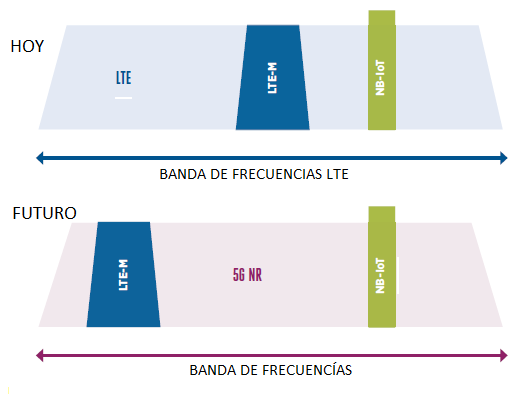
\includegraphics[scale=1]{Figures/5G NR con LTE-M y NB-IoT en banda}
\decoRule
\caption[5G NR con LTE-M y NB-IoT en banda]{5G NR con LTE-M y NB-IoT en banda}
\label{fig:5gnr}
\end{figure}

En la \textit{Tabla~\ref{tab:tecIoT}} se pueden encontrar características de estas tecnologías antes descritas, tales como la banda de frecuencia a la que operan y su tasa de transmisión y si bien pareciera que la diferencia entre ambas tecnologías es sutil, en realidad, ésta marca una clara pauta en el servicio que pueden brindar. \newline

\begin{table}
\caption{Características de las tecnologías de red para IoT en la red celular}
\label{tab:tecIoT}
\centering
\begin{tabular}{|p{0.6in}|p{0.6in}|p{0.4in}|p{0.6in}|p{0.4in}|p{0.5in}|p{0.8in}|p{0.4in}|} \\ 
\textbf{\textit{Tecnología}} & \textbf{\textit{Banda de Frecuencia}} & \textbf{\textit{Rango}} & \textbf{\textit{Tasa de transmisión}} & \textbf{\textit{Vida de la batería}} & \textbf{\textit{Topología}} & \textbf{\textit{Estandarización}} & \textbf{\textit{Grupo}} \\ 
\textbf{NB-IoT}  & \footnotesize{ 450 MHZ -- 3.5 GHz (Espectro de 2G/3G/4G) } & \footnotesize{ 10-15 km } & \footnotesize{ 250 kbps } & \footnotesize{ 10+ años } & \footnotesize{ Estrella } & \footnotesize{ Abierto } & \footnotesize{ 3GPP } \\ \hline
\textbf{eMTC}  & \footnotesize{ 450 MHZ -- 3.5 GHz (El mismo que LTE) } & \footnotesize{ 10-15 km } & \footnotesize{ 1 Mbps } & \footnotesize{ 10+ años } & \footnotesize{ Estrella } & \footnotesize{ Abierto } & \footnotesize{ 3GPP } \\
\end{tabular}

\end{table}


En la \textit{Figura~\ref{fig:lpwa}} se puede observar otra comparación entre ambas tecnologías pero en esta ocasión desde la perspectiva de las aplicaciones a la que tanto NB-IoT y/o LTE-M estarían dando servicio preferentemente. A la izquierda de la \textit{Figura~\ref{fig:lpwa}} tenemos las aplicaciones LPWAN a las que NB-IoT daría servicio que coinciden con una menor velocidad de transferencia y mayor tolerancia a la latencia mientras que a la derecha se aglomeran las aplicaciones que requieren una comunicación en tiempo real y una mayor tasa de transmisión, aplicaciones a las que estaría dando servicio preferentemente la tecnología eMTC. \newline

Se decidió entonces concentrarse en la tecnología NB-IoT puesto que la totalidad de los servicios que se considerarán en nuestro sistema pueden situarse a la izquierda de la \textit{Figura~\ref{fig:lpwa}}, donde se presenta una mínima movilidad de los dispositivos, por ejemplo el control de la iluminación y el control dinámico de los semáforos podríamos colocarlos en \textit{Iluminación pública y Ciudades inteligentes }respectivamente, mientras que el monitoreo de consumo energético y el de la condición del aire podrían corresponder a \textit{Medidores inteligentes}, de manera que quizá el único servicio que se encontraría en los límites de la tecnología NB-IoT sería el de detección de cortes en el suministro energético, el cual en \parencite{NetTrafficIoT} establece que requeriría de una mínima latencia.\newline


\begin{figure}[th]
\centering
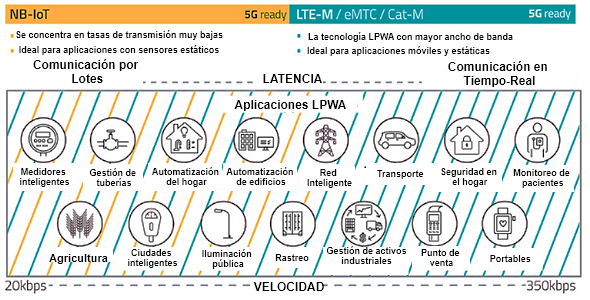
\includegraphics[scale=1]{Tecnología líder para el caso de uso LPWA}
\decoRule
\caption[Tecnologías líder para el caso de uso LPWA]{Tecnologías líder para el caso de uso LPWA, [Fuente: https://www.iotforall.com/cellular-iot-explained-nb-iot-vs-lte-m/]}
\label{fig:lpwa}
\end{figure}

Con esta argumentación se explica la decisión de haber seleccionado la tecnología de red NB-IoT como de la que partiremos para después agregar mejoras propuestas en otros trabajos y diseñar un modelo de sistema para la simulación en el que con modelos de tráfico adecuados se puedan medir los indicadores clave de rendimiento y determinar si la calidad de servicio esperada para los servicios LPWAN seleccionados se cumplirán en redes celulares 5G.

La \textit{Figura~\ref{fig:5gqos}} muestra las distintas tecnologías con las que estaría trabando 5G NR para poder brindar servicio al amplio espectro de casos de uso de MTC \parencite{5GAmericas}. La tecnología NB-IoT podemos situarla en las frecuencias de operación baja y con un una tolerancia al retardo mayor que la mayoría de las demás tecnologías.

\begin{figure}[th]
\centering
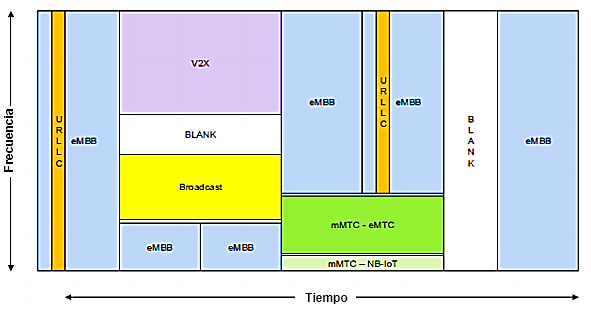
\includegraphics[scale=1]{5G NR soportará múltiples servicios con distintos requerimiento de QoS}
\decoRule
\caption[5G NR soportará múltiples servicios con distintos requerimiento de QoS]{5G NR soportará múltiples servicios con distintos requerimiento de QoS}
\label{fig:5gqos}
\end{figure}

\subsection{Análisis del estándar NB-IoT} 

En particular, el estándar NB-IoT fue especificado en el reporte TR 45.820 (\textit{release} 13) de la 3GPP \parencite{3GPP2019}. Los parámetros fundamentales son:\newline

Para el enlace de subida (\textit{uplink}), como su nombre lo indica, tiene un ancho de banda estrecho de 180 kHz y un espacio de sub-portadora de 3.75 kHz (ancho de banda de transmisión mínimo para un dispositivo). Por lo tanto puede asignar 48 sub-portadoras [\textit{véase Figura~\ref{fig:NBIoT}}].

\begin{figure}[th]
\centering
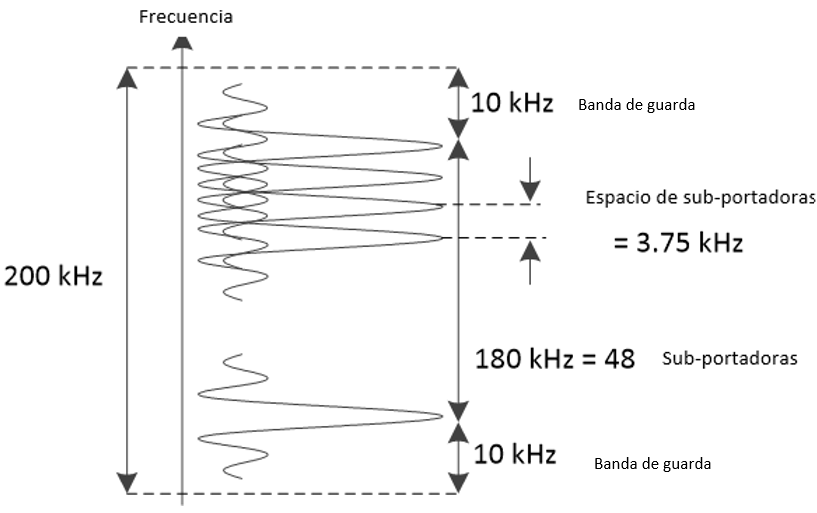
\includegraphics[scale=1]{Estructura de ancho de banda y subportadoras en NB-IoT}
\decoRule
\caption[Estructura de ancho de banda y subportadoras en NB-IoT.]{Estructura de ancho de banda y subportadoras en NB-IoT.}
\label{fig:NBIoT}
\end{figure}

El enlace de bajada (\textit{downlink}), se conserva la estructura de transmisión del enlace descendente de \textit{Long Term Evolution} (LTE) con un espaciado de sub-portadora de 15 kHz.\newline

Por lo tanto, NB-IoT puede proporcionar velocidades de datos de casi 250 kb / s en el enlace descendente y 20 kb / s en el enlace ascendente.\newline

En esta especificación también se detallan algunos aspectos de tráfico en términos de los tamaños de paquetes que se esperan para NB-IoT. Se definen cuatro tipos de aplicaciones de tráfico diferentes.

\subsubsection{Reportes autónomos móviles (MAR, \textit{Mobile Autonomous Reporting}}
\subsubsection{Informes de excepción}
Se espera que muchas aplicaciones de tipo sensor monitoreen una condición física y activen un informe de excepción cuando se detecte un evento. Estos eventos serán, en general, raros y ocurrirán cada pocos días, meses o incluso años. Ejemplos de tales aplicaciones incluyen detectores de alarma de humo, notificaciones de fallas de energía de medidores inteligentes, notificaciones de manipulación, etc.\newline

Para el análisis de latencia, se supone que los informes de excepción MAR tienen una carga útil de la aplicación de enlace ascendente de 20 bytes. Se requiere que dichos informes se entreguen casi en tiempo real, con un objetivo de latencia de 10 segundos.\newline

Para cada informe de enlace ascendente generado (es decir, el 100\% de los informes de excepción de enlace ascendente), también se supone que la aplicación enviará un ACK de aplicación de enlace descendente. El tamaño del tamaño ACK de la capa de aplicación es cero. El tamaño total del paquete (por encima del equivalente de la capa SNDCP) es la sobrecarga debida COAP / DTLS / UDP / IP.\newline

\subsubsection{Informes periódicos}

Se espera que los informes periódicos de enlace ascendente sean comunes para aplicaciones de IoT celular como informes de medición de servicios inteligentes (gas / agua / electricidad), agricultura inteligente, entorno inteligente, etc. El modelo de tráfico de informes de enlace ascendente periódico MAR se utiliza en simulaciones a nivel de sistema para análisis de capacidad.\newline

Distribución del tamaño de la carga útil de la aplicación. UL. Sigue una distribución de Pareto con parámetro alfa = 2.5 y tamaño mínimo de carga útil de la aplicación = 20 bytes con un corte de 200 bytes, es decir, las cargas superiores a 200 bytes serán limitadas a 200 bytes.\newline

Se supone un ACK de capa de aplicación DL para un evento de informe periódico de enlace ascendente en el 50\% de los informes periódicos UL MAR generados. Se supone que el tamaño de la carga útil ACK del enlace descendente de la aplicación es de 0 bytes. El tamaño total del paquete (superior al equivalente de la capa SNDCP) es la sobrecarga debida a COAP / DTLS / UDP / IP y se envía inmediatamente después de que la estación base recibe con éxito un paquete UL de aplicación.\newline

Entonces, una vez revisadas estas clasificaciones de tráfico compatibles para NB-IoT, se procede a agrupar estos tipos de tráfico con los escenarios que se consideraron en la \textit{Tabla 8} de la sección anterior, de tal manera que se establezcan las condiciones base de un ambiente NB-IoT de acuerdo a los servicios seleccionados (secXXXX).\newline

La adición de la columna ``Tamaños de paquete'' para la \textit{Tabla~\ref{tab:}} se da en la \textit{Tabla~\ref{tab:}}\newline

\begin{table}
\caption{Caracterización del tráfico de paquetes en aplicaciones seleccionadas para la simulación.}
\label{tab:trafpkt}
\centering
\begin{tabular}{*{2}{m{7cm}}}\\ 
\textbf{\textit{Servicio}} & \textbf{Tamaño de paquetes} \\ 
\textit{Control de iluminación (Smart City) } & \footnotesize{ Activación aleatoria \textbf{UL}: 20 bytes \textit{payload} \textbf{DL}: ACK de 0 bytes } \\ \hline 
\textit{Monitoreo del consumo de agua y electricidad en la ciudad (Smart City) } & \footnotesize{ Activación periódica \textbf{UL}: distribución de Pareto con parámetro alfa = 2.5 y tamaño mínimo de carga útil de la aplicación = 20 bytes con un corte a 200 bytes \textbf{DL}: ACK de 0 bytes 50\% de las veces. } \\ \hline 
\textit{Detección de terremotos (Smart Environment)}  & \footnotesize{ Activación aleatoria \textbf{UL}: 20 bytes \textit{payload} \textbf{DL}: ACK de 0 bytes } \\ \hline 
\textit{Monitoreo de contaminación del aire (Smart Environment) } & \footnotesize{ Activación periódica \textbf{UL}: distribución de Pareto con parámetro alfa = 2.5 y tamaño mínimo de carga útil de la aplicación = 20 bytes con un corte a 200 bytes \textbf{DL}: ACK de 0 bytes 50\% de las veces. } \\ \hline 
\textit{Control dinámico de semáforos (Smart Transport and Mobility)}  & \footnotesize{ Activación aleatoria \textbf{UL}: distribución de Pareto con parámetro alfa = 2.5 y tamaño mínimo de carga útil de la aplicación = 20 bytes con un corte a 200 bytes \textbf{DL}: ACK de 0 bytes 50\% de las veces. } \\ \hline 
\textit{Genérico}  & \footnotesize{ Activación aleatoria \textbf{UL}: 20 bytes \textit{payload} \textbf{DL}: ACK de 0 bytes } \\  
\end{tabular}
\end{table}


%----------------------------------------------------------------------------------------
%	SECTION 
%----------------------------------------------------------------------------------------

\section{INDICADORES CLAVE DE RENDIMIENTO (KPIs)}

Hay muchas formas de medir el rendimiento de una red, por medio de sus características se pueden definir los indicadores clave de rendimiento para la evaluación integral, precisa y eficiente de las tecnologías de red 5G.\newline

Con la profundización de la investigación de la tecnología 5G, se puede prever que habrá nuevos indicadores de evaluación. El diseño de estos indicadores directamente medibles, por un lado, necesita combinar las características de los nuevos servicios, y por otro lado, debe aprender completamente de la experiencia de los KPI clásicos de generaciones anteriores como lo son: el \textit{throughput, }dada una\textit{ }probabilidad de salida y la latencia. La densidad de conexión, la densidad de volumen de tráfico y el consumo de energía son nuevos KPI introducidos por las redes 5G/IoT \parencite{WirelessSim}.\newline

Para cumplir con el conjunto de requisitos de mMTC, NB-IoT debe admitir principalmente cuatro indicadores clave de rendimiento (KPI).\newline

\begin{enumerate}
\item  Vida útil de la batería del dispositivo más allá de 10 años, suponiendo una capacidad de energía almacenada de 5 Wh.
\item  Densidad de conexión masiva de hasta 1M dispositivos por km cuadrado en un entorno urbano.
\item  Latencia de como máximo 10 s.
\item  Una tasa máxima alcanzable de hasta 200kbps (subida).
\end{enumerate}

El análisis fundamental del simulador contemplará como métricas de desempeño a la compensación entre la tasa máxima alcanzable y la densidad de usuarios atendidos en términos de una calidad de servicio QoS. Esta QoS dependerá de los cuatro principales KPIs para mIoT.\newline

Por lo tanto, de acuerdo a las métricas que serán consideradas, los KPIs a considerar son: la tasa máxima alcanzable y la densidad de usuarios, sin embargo durante las investigaciones que hemos realizado en la literatura científica no hemos encontrado ningún artículo que proponga un modelo de sistema que alcance el KPI de soportar hasta 1 millón de dispositivos. Por lo que para esta métrica se buscará un diseño de sistema tal que a un determinado tope de usuarios se logre una óptima tasa UL, es decir, el dimensionamiento de la red.

%----------------------------------------------------------------------------------------
%	SECTION 
%----------------------------------------------------------------------------------------

\section{ANÁLISIS DE MODELOS PARA LA EVALUACIÓN DE REDES 5G/IoT}
\subsection{MODELO DE DESPLIEGUE DE BSs Y UEs}
\subsection{MODELO DE CANAL}
\subsection{ESQUEMA DE ACCESO MÚLTIPLE AL MEDIO}
\subsection{MODELOS DE TRÁFICO}


